\documentclass[11pt,a4paper]{article}
\usepackage[T1]{fontenc}
\usepackage[utf8]{inputenc}
\usepackage[margin=1in]{geometry}
\usepackage{amsmath,amssymb,amsthm}
\usepackage{mathpartir}
\usepackage{stmaryrd}
\usepackage{booktabs}
\usepackage{tabularx}
\usepackage{array}
\usepackage{enumitem}
\usepackage{listings}
\usepackage{xcolor}
\usepackage[expansion=false]{microtype}
\usepackage{tikz}
\usetikzlibrary{arrows.meta,positioning,fit,calc}
\usepackage[htt]{hyphenat}
\usepackage[hidelinks,pdftitle={K1NDL1NG: a parser and a normaliser for the kernel of rholang}]{hyperref}
\setlength{\emergencystretch}{3em}

\newcommand{\code}[1]{\texttt{#1}}
\newcommand{\Kind}{\textsc{K1ndl1ng}}
\newcommand{\Camp}{\textsc{CampF1R3}}
\newcommand{\Rhobots}{\textsc{Rhobots}}
\newcommand{\MUST}{\textsc{must}}
\newcommand{\MUSTNOT}{\textsc{must not}}
\newcommand{\SHOULD}{\textsc{should}}
\newcommand{\SHOULDNOT}{\textsc{should not}}
\newcommand{\MAY}{\textsc{may}}
\newcommand{\enc}[1]{\llbracket #1 \rrbracket}
\newcommand{\rr}{\rightharpoonup}

\theoremstyle{definition}
\newtheorem{definition}{Definition}[section]
\newtheorem{requirement}[definition]{Requirement}
\newtheorem{decision}[definition]{Decision}
\newtheorem{obligation}[definition]{Obligation}
\newtheorem{remark}[definition]{Remark}
\theoremstyle{plain}
\newtheorem{proposition}[definition]{Proposition}
\newtheorem{lemma}[definition]{Lemma}

\lstset{
  basicstyle=\ttfamily\footnotesize,
  columns=fullflexible,
  keepspaces=true,
  breaklines=true,
  frame=leftline,
  framesep=6pt,
  xleftmargin=8pt,
  rulecolor=\color{black!30},
  showstringspaces=false,
}

\title{\textbf{\Kind}\\[1mm]
\large A parser and a normaliser for the kernel of rholang\\
served by \Camp, as composable crates\\[2mm]
\normalsize Specification v0.2}
\author{F1R3FLY.io}
\date{17 September 2026}

\begin{document}
\maketitle
\begin{abstract}
\noindent
\Camp{} is a store: it holds data and continuations at channels and fires a
matching step. It deliberately knows nothing about processes, and lists the
parser and the normaliser as non-goals. \Rhobots{} is an immersive editor for
pure rho on Apple Vision Pro, and needs the same terms in the same shapes, on a
device where a C-backed parser is unwelcome. This document specifies the two
components that fill those holes, as \emph{separate, independently usable}
crates: \code{k1ndl1ng-parse}, which takes text to a typed abstract syntax tree,
and \code{k1ndl1ng-norm}, which takes that tree to a representation with de
Bruijn indices and ordered parallel components, from which name equality is a
byte comparison. Both are built over a shared \code{k1ndl1ng-ast}, neither
depends on the other's consumers, and neither reduces anything. Composed with
\Camp{} and an interpreter, they make an executive
(Section~\ref{sec:executive}). The specification fixes the nomenclature
(Section~\ref{sec:nomen}) and the grammar (Section~\ref{sec:lang}); the tree
(Section~\ref{sec:ast}), the parser (Section~\ref{sec:parse}) and the normaliser
(Section~\ref{sec:norm}) crate by crate; the error model
(Section~\ref{sec:errors}), the editor services \Rhobots{} needs
(Section~\ref{sec:editor}), and the portability, determinism and performance
requirements (Sections~\ref{sec:perf}--\ref{sec:wasm}).
Key words \MUST, \MUSTNOT, \SHOULD, \MAY{} are used in the sense of RFC~2119.
\end{abstract}
\tableofcontents
%======================================================================
\section{Purpose and scope}\label{sec:purpose}

\subsection{The gap}

The \Camp{} specification (v0.1) covers the store and the matching step, and is
explicit that ``the parser and the normaliser are non-goals''. Its WebAssembly
build is instantiated at $C=A=K=\code{Bytes}$ with a placeholder
\code{ExactBytes} matcher, precisely so that the store can be exercised in a
browser \emph{before} a parser is available. That placeholder is the hole this
document fills.

The same hole is open on the other side. \Rhobots{} renders pure rho as robots
exchanging payloads, with the $z$ axis carrying continuations. It needs to turn
typed text into terms, terms back into text, and terms into a scene graph with
stable identity across edits; and it needs all of that on a headset, in a build
where linking two and a half megabytes of generated C is a poor use of the
budget.

\subsection{What exists today}

\begin{center}
\begin{tabularx}{\linewidth}{@{}l>{\raggedright\arraybackslash}X@{}}
\toprule
Component & State\\
\midrule
\code{rholang-parser} (\code{rholang-rs}, rev \code{02cef80}) &
Tree-sitter front end for the whole of rholang, pinned as a git dependency by
\code{f1r3node-rust}. The generated \code{src/parser.c} is 2.75\,MB; the crate
carries an arena-allocated AST (\code{ast.rs}, 913 lines) and a traversal layer
(1851 lines).\\
\code{rholang-parser} on \code{wasm32} &
The tree-sitter backend is compiled out, and \code{parser\_wasm.rs} substitutes a
stub whose \code{parse} returns \code{Validated::Good(vec![])}. Every program is
silently the empty process.\\
\code{rholang/\dots/compiler} (\code{f1r3node-rust}) &
\code{Compiler::source\_to\_adt} plus a normaliser of 23 per-construct visitors,
producing \code{models::rhoapi::Par}. Depends on \code{models}, \code{prost} and
the rest of the workspace.\\
\code{models/\dots/sorter} &
Score-tree canonical ordering over \code{Par}, 15 sort matchers, the basis of the
Blake2b-256 content hashes \code{rspace++} already computes.\\
\code{rho-pure-eval} &
Deterministic evaluator for a subset of \code{Expr}, used for \code{where} guards
and match-case guards. 1042 lines.\\
\bottomrule
\end{tabularx}
\end{center}

\begin{remark}[Why not simply reuse the tree-sitter front end]
Three reasons, in order of weight. First, it does not work on the target: the
\code{wasm32} path is a stub that returns an empty AST rather than an error, so a
\Rhobots{} build or a browser \Camp{} demo would run, and would be wrong.
Second, it parses the whole language, which is the wrong size for a store whose
kernel is six constructors; grammar surface that nothing downstream can execute
is surface that must still be diagnosed, printed and tested. Third, the
canonical form and the content hash --- the things \Camp{} actually requires of
its caller --- live in \code{models}, behind \code{prost}, \code{bincode} and the
workspace, none of which \Camp{} is permitted to depend on.
\end{remark}

\begin{remark}[What is kept]
\Kind{} is not a rejection of that work. The grammar of
\code{rholang-tree-sitter} is normative for surface syntax: where \Kind{} accepts
a form, it \MUST{} accept it with the same spelling and the same meaning, so that
a kernel program is a rholang program. The AST shape (\code{Proc}, \code{Name},
\code{Bind}, \code{Source}, \code{SendType}) is followed where the kernel
overlaps it, so that a later merge or replacement is mechanical rather than a
redesign. The tree-sitter grammar and this crate are cross-checked by
differential testing (Section~\ref{sec:testing}).
\end{remark}

\subsection{Nomenclature}\label{sec:nomen}

Three words are used precisely throughout, and nowhere interchangeably.

\begin{center}
\begin{tabularx}{\linewidth}{@{}l>{\raggedright\arraybackslash}X@{}}
\toprule
Term & Meaning in this document\\
\midrule
\emph{Parsing} & Taking a textual representation to a typed abstract syntax
tree. Nothing more: no binder analysis, no reordering, no equality. The output
is a faithful tree over the source, with spans.\\
\emph{Normalisation} & Taking that tree to a representation that uses de Bruijn
indices and orders the components of a parallel composition, together with the
encoding and content hash that follow from it. This is what makes name equality
cheap, and it is the whole reason the stage exists.\\
\emph{Reduction} & Execution: firing communications, including running a term to
a normal form in the operational sense. No crate in this document performs any
reduction.\\
\bottomrule
\end{tabularx}
\end{center}

\begin{remark}[Two senses of ``normal form'']
\Camp{} uses \emph{normal form} for a store state in which no match remains.
That is a property of a store, reached by reduction. The \emph{normal form} of
this document is a property of a term, reached by normalisation, and no term is
ever reduced to get it. Where confusion is possible, this document says
\emph{normal form of a term} or \emph{quiescent store}.
\end{remark}

\begin{decision}[One document, two crates]\label{dec:twocrates}
Parsing and normalisation are separate components and are specified as separate
crates. A consumer that only needs a tree --- an editor, a formatter, a syntax
highlighter, a gesture interface building terms by hand --- \MUSTNOT{} be made
to link a normaliser, and a consumer that only needs terms --- an interpreter, a
matcher, a store client fed by the wire rather than by text --- \MUSTNOT{} be
made to link a lexer. Section~\ref{sec:arch} gives the boundary; the remainder of
the document is organised crate by crate.
\end{decision}

\subsection{Goals}

\begin{enumerate}[nosep,leftmargin=1.6em]
\item \textbf{Separable.} Each crate is usable, testable and versionable on its
  own, and the dependency graph is a line, not a cycle
  (Requirement~\ref{req:acyclic}).
\item \textbf{Composable.} Parser, normaliser, \Camp{} and an interpreter
  assemble into an executive with no glue beyond type instantiation, on a
  headset, in a browser or on a node (Section~\ref{sec:executive}).
\item \textbf{Small.} One kernel, six process constructors and two name
  constructors at level~K0; each crate in the low thousands of lines, with a
  \code{wasm32} code-size budget three orders of magnitude under the generated
  parser it replaces (Section~\ref{sec:perf}).
\item \textbf{Tight.} Parse, normalise and hash in one pass each, over an arena,
  with no intermediate \code{String} and no regular expression engine.
\item \textbf{Portable.} \code{wasm32-unknown-unknown} is a \MUST{} target, and
  a first-class one: no stubs, no silent degradation, no C, no
  \code{getrandom}, no clock.
\item \textbf{Two-way.} Trees print back to source, and normal forms print back
  to trees. \Rhobots{} builds terms by gesture and must be able to show and
  export them as text.
\end{enumerate}

\subsection{Non-goals}

Reduction in any form, matching, scheduling, cost accounting, storage,
consensus, the name registry, unforgeable-name derivation compatible with a
particular deploy scheme, the \code{Expr} layer of rholang beyond the guard
subset, and language-definition (DDL) syntax. Each is named where it touches an
interface, and each belongs to another crate. A term here is data.

\begin{decision}[Substitution belongs to the normaliser]\label{dec:subst}
Capture-avoiding substitution and de Bruijn shifting are \emph{included} in
\code{k1ndl1ng-norm}, though a substitution is not a normalisation. They are
operations on the de Bruijn representation, they are small and total given that
representation, and an interpreter that had to reimplement them against someone
else's indices would be reimplementing the normaliser's invariants. Applying a
substitution is not reduction: the interpreter decides what to substitute and
when.
\end{decision}

\subsection{Sources}

\begin{itemize}[nosep]
\item Store interface and its obligations on the caller: the \Camp{}
  specification v0.1, especially the hash discipline, the dependency allowlist
  and the determinism profiles.
\item Surface syntax: \code{rholang-tree-sitter/grammar.js} and
  \code{rholang-parser/src/ast.rs}, \code{rholang-rs} rev \code{02cef80}.
\item Canonical order and content hashing: \code{models/src/rust/rholang/sorter},
  \code{f1r3node-rust}, branch \code{feature/cost-accounted-rho}.
\item Guard sublanguage: \code{rho-pure-eval}, same branch.
\item Consumer requirements: \emph{Rhobots in Space} v0.6.
\item Calculus: the rho calculus as presented in the f1r3lang papers in
  \code{publications}; reflection, and the laws $@{*x} = x$ and $*@P \equiv P$.
\end{itemize}

%======================================================================
\section{The language}\label{sec:lang}

\subsection{Three levels}

The kernel is stratified, so that a consumer can state exactly what it accepts
and a diagnostic can say exactly why a form was rejected.

\begin{center}
\begin{tabularx}{\linewidth}{@{}l>{\raggedright\arraybackslash}X>{\raggedright\arraybackslash}p{0.23\linewidth}@{}}
\toprule
Level & Adds & Consumer\\
\midrule
K0 \emph{pure rho} & \code{Nil}, par, monadic send, monadic receive on a name
variable, unquote, quote & \Rhobots{} v1\\
K1 \emph{store kernel} & polyadic send and receive, joins (\code{\&}),
persistent receive (\code{<=}), peek (\code{<<-}), persistent send (\code{!!}),
name patterns with wildcards and free variables, \code{new}, sequential
receipts (\code{;}) as sugar & \Camp, node adapter\\
K2 \emph{guards} & \code{where} clauses on receipts, over the
\code{rho-pure-eval} expression subset & deferred, feature-gated\\
\bottomrule
\end{tabularx}
\end{center}

\begin{requirement}[Level is a parser parameter]\label{req:level}
The parser \MUST{} take the accepted level as an explicit parameter, \MUST{}
reject forms above that level with a diagnostic naming the level that would
accept them, and \MUSTNOT{} silently accept them. K0 and K1 \MUST{} be
implemented in v1. K2 \MUST{} be behind the \code{guards} cargo feature, off by
default, and \MAY{} be deferred to v1.1.
\end{requirement}

\begin{decision}[Why K0 is not merely ``K1 with one binder'']
\Rhobots{} renders a robot per constructor. Arity, joins, persistence and peek
each need a distinct physical form, and the spec reserves but does not fix them.
Making K0 a real level, checkable by the parser, lets the editor refuse to load
a term it cannot draw, rather than drawing it wrongly.
\end{decision}

\subsection{Lexical structure}

\begin{center}
\begin{tabularx}{\linewidth}{@{}l>{\raggedright\arraybackslash}X@{}}
\toprule
Class & Definition\\
\midrule
Identifier & \code{[a-zA-Z\_][a-zA-Z0-9\_']*}, not a reserved word. ASCII only in
v1; the lexer \MUST{} reject non-ASCII identifier bytes with a diagnostic rather
than accept them silently.\\
Wildcard & \code{\_} standing alone.\\
Punctuation & \code{( ) \{ \} @ * ! !! | \& ; , <- <= <<- new in}\\
Comment & \code{//} to end of line; \code{/*} \ldots \code{*/}, not nested.\\
Whitespace & space, tab, carriage return, line feed. No layout rule.\\
Reserved & \code{Nil new in for where contract match select let if else bundle
bundle0 bundle+ bundle- true false not and or matches}\\
\bottomrule
\end{tabularx}
\end{center}

\begin{requirement}[Reserved words are reserved at every level]
Words reserved for constructs above the accepted level \MUST{} be lexed as
keywords and \MUST{} produce a ``not in this kernel'' diagnostic, never an
identifier. This is what keeps a kernel program a rholang program, and keeps a
future level from silently changing the meaning of an old term.
\end{requirement}

\subsection{Grammar}

Nonterminals are italic; terminals are typeset in \code{typewriter}. The suffix
$^{K1}$ marks a production available only at K1 and above, and $^{K2}$ at K2.

\[
\begin{array}{lcll}
\mathit{Proc} &::=& \code{Nil} & \text{the inert process}\\
 &\mid& \mathit{Proc}\ \code{|}\ \mathit{Proc} & \text{parallel composition}\\
 &\mid& \mathit{Name}\ \mathit{Bang}\ \code{(}\ \mathit{Proc}^{*,}\ \code{)} & \text{send}\\
 &\mid& \code{for}\ \code{(}\ \mathit{Receipts}\ \code{)}\ \code{\{}\ \mathit{Proc}\ \code{\}} & \text{receive}\\
 &\mid& \code{*}\ \mathit{Name} & \text{unquote}\\
 &\mid& \code{new}\ \mathit{Id}^{+,}\ \code{in}\ \code{\{}\ \mathit{Proc}\ \code{\}} & \text{name creation}^{K1}\\
 &\mid& \code{(}\ \mathit{Proc}\ \code{)} &\\[2pt]
\mathit{Name} &::=& \mathit{Id} \mid \code{\_}^{K1} \mid \code{@}\ \mathit{Proc} &\\[2pt]
\mathit{Bang} &::=& \code{!} \mid \code{!!}^{K1} &\\[2pt]
\mathit{Receipts} &::=& \mathit{Receipt}\ (\code{;}\ \mathit{Receipt})^{*\,K1} &\\
\mathit{Receipt} &::=& \mathit{Bind}\ (\code{\&}\ \mathit{Bind})^{*\,K1}\ (\code{where}\ \mathit{Guard})^{?\,K2} &\\
\mathit{Bind} &::=& \mathit{NamePat}^{*,}\ \code{<-}\ \mathit{Name} & \text{linear}\\
 &\mid& \mathit{NamePat}^{*,}\ \code{<=}\ \mathit{Name} & \text{persistent}^{K1}\\
 &\mid& \mathit{NamePat}^{*,}\ \code{<<-}\ \mathit{Name} & \text{peek}^{K1}\\[2pt]
\mathit{NamePat} &::=& \mathit{Id} \mid \code{\_}^{K1} \mid \code{@}\ \mathit{ProcPat}^{K1} &\\
\mathit{ProcPat} &::=& \text{a \emph{Proc} with free identifiers and }\code{\_}^{K1} &
\end{array}
\]

\noindent
$X^{*,}$ is a possibly empty comma-separated list, $X^{+,}$ a non-empty one.
At K0, a $\mathit{Bind}$ has exactly one $\mathit{NamePat}$, which is an
$\mathit{Id}$; a send has exactly one argument; $\mathit{Receipts}$ is a single
$\mathit{Bind}$ with \code{<-}.

\begin{center}
\begin{tabular}{@{}llll@{}}
\toprule
Precedence & Form & Associativity & Note\\
\midrule
lowest & \code{|} & left, but see below & flattened, then sorted\\
 & \code{for}, \code{new} & --- & body is brace-delimited\\
 & \code{!}, \code{!!} & --- & argument list is paren-delimited\\
highest & \code{*}, \code{@} & prefix, right & \code{*@P} and \code{@*x} are legal\\
\bottomrule
\end{tabular}
\end{center}

\begin{remark}[Associativity of \code{|} is not observable]
The parser \MAY{} read \code{|} left-associated, but the tree \MUST{} record
parallel composition as a flat sequence of components in source order
(Requirement~\ref{req:flatpar}); ordering that sequence is the normaliser's
business, not the parser's. Parsing \code{|} into a right-leaning spine of
\code{Par\{left,right\}} nodes, as the tree-sitter AST does, forces every
consumer to re-flatten.
\end{remark}

\subsection{Out of scope, explicitly}

Ground literals of every sort, collections, methods, \code{contract},
\code{match}, \code{select}, \code{let}, \code{if}/\code{else}, bundles,
\code{!?} and \code{?!} sources, method-call source sugar, \code{VarRef}
(\code{=x}), logical connectives in patterns (\code{/\textbackslash},
\code{\textbackslash/}, \code{\~{}}), \code{matches}, and simple types. All are
reserved words or reserved punctuation; all produce a level diagnostic.

\begin{obligation}[Connectives in patterns]\label{obl:conn}
\Camp{} treats patterns as opaque and delegates to a caller-supplied matcher, so
nothing in the store forbids connectives. They are excluded from v1 because the
kernel's matcher (a separate deliverable) is specified for spatial patterns with
free variables and wildcards only. If the node adapter is to serve
\code{f1r3node} terms in general, connectives are the first extension, and the
grammar above reserves their tokens for that purpose.
\end{obligation}

\subsection{Congruence}

\begin{definition}[Structural congruence]\label{def:cong}
$\equiv$ is the least congruence on $\mathit{Proc}$ such that
$(\mathit{Proc},\code{|},\code{Nil})$ is a commutative monoid, $\alpha$-equivalent
terms are identified, and $*@P \equiv P$. Name equivalence $\equiv_N$ is the
least congruence on $\mathit{Name}$ such that $@P \equiv_N @Q$ whenever
$P\equiv Q$, and $@{*x} \equiv_N x$.
\end{definition}

\begin{requirement}[Congruence is decided, not approximated]\label{req:cong}
For every pair of kernel terms $P,Q$, $\enc{P}=\enc{Q}$ if and only if
$P\equiv Q$, where $\enc{-}$ is the normal-form encoding of
Section~\ref{sec:norm}. Equality of terms, equality of encodings and equality of
content hashes (modulo collision) \MUST{} agree.
\end{requirement}

\begin{remark}
Requirement~\ref{req:cong} is what \Camp{} is really asking for when it says the
caller supplies content hashes and that ``equal values \MUST{} have equal
hashes''. Two channels that are congruent but encode differently would split one
channel into two, and messages would never meet. This is the single most
load-bearing property in this document, and Section~\ref{sec:norm} proves it for
the kernel.
\end{remark}
%======================================================================
\section{Architecture}\label{sec:arch}

\subsection{The crates}

\begin{center}
\resizebox{\linewidth}{!}{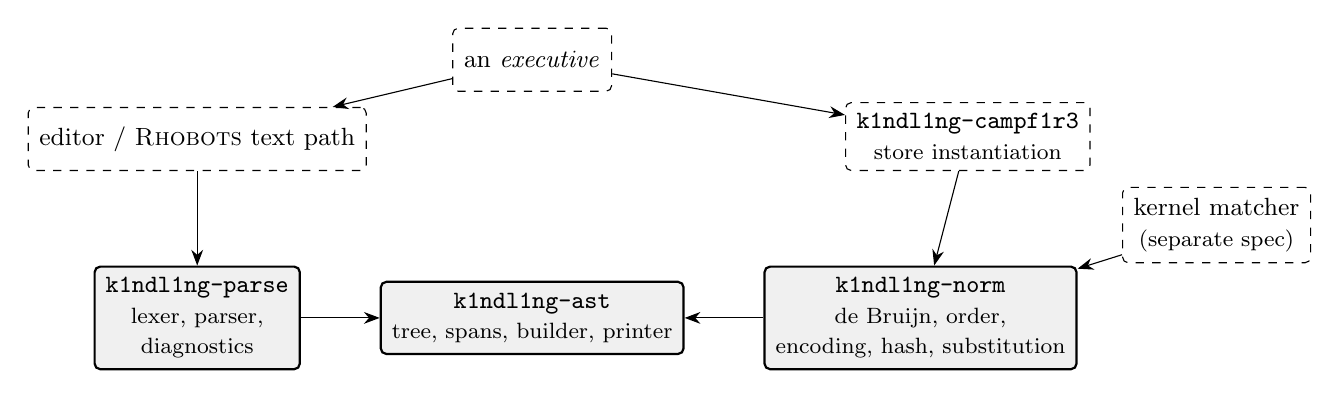
\begin{tikzpicture}[
  box/.style={draw,rounded corners=2pt,align=center,font=\small,minimum height=8mm,inner sep=4pt},
  core/.style={box,fill=black!6,thick},
  ext/.style={box,dashed},
  dep/.style={-{Stealth[length=2mm]},thin}]
\node[core] (ast) {\code{k1ndl1ng-ast}\\ \footnotesize tree, spans, builder, printer};
\node[core,left=10mm of ast] (parse) {\code{k1ndl1ng-parse}\\ \footnotesize lexer, parser,\\ \footnotesize diagnostics};
\node[core,right=10mm of ast] (norm) {\code{k1ndl1ng-norm}\\ \footnotesize de Bruijn, order,\\ \footnotesize encoding, hash, substitution};
\node[ext,above=12mm of parse] (edit) {editor / \Rhobots{} text path};
\node[ext,above=12mm of norm,xshift=6mm] (glue) {\code{k1ndl1ng-campf1r3}\\ \footnotesize store instantiation};
\node[ext,above=12mm of ast,yshift=12mm] (exec) {an \emph{executive}};
\node[ext,below right=2mm and 4mm of glue] (match) {kernel matcher\\ \footnotesize (separate spec)};
\draw[dep] (parse) -- (ast); \draw[dep] (norm) -- (ast);
\draw[dep] (edit) -- (parse); \draw[dep] (glue) -- (norm); \draw[dep] (match) -- (norm);
\draw[dep] (exec) -- (edit); \draw[dep] (exec) -- (glue);
\end{tikzpicture}}
\end{center}

\begin{center}
\begin{tabularx}{\linewidth}{@{}l>{\raggedright\arraybackslash}X>{\raggedright\arraybackslash}p{0.21\linewidth}@{}}
\toprule
Crate & Owns & Depends on\\
\midrule
\code{k1ndl1ng-ast} & The typed tree: node types, arena, spans, trivia, node
identity, traversal, the construction API, and printing a tree back to text.
This is the vocabulary the other two share.
& \code{core}, \code{alloc}\\
\code{k1ndl1ng-parse} & Lexer, parser, error model, recovery, fragment parsing
and splice. Text in, tree out.
& \code{k1ndl1ng-ast}\\
\code{k1ndl1ng-norm} & Binder resolution, de Bruijn assignment, ordering of
parallel components, the normal form, its encoding, content hashing,
substitution and shifting, and queries over normal forms.
& \code{k1ndl1ng-ast}\\
\code{k1ndl1ng-wasm} & \code{wasm-bindgen} bindings, one module per crate
behind cargo features, so a browser build can take the parser without the
normaliser or the reverse.
& both, optional\\
\code{k1ndl1ng-campf1r3} & Instantiation of \Camp's \code{Channel},
\code{Datum}, \code{Pattern} and \code{Cont} at normal-form types
(Section~\ref{sec:glue}). A glue crate, deliberately trivial.
& \code{k1ndl1ng-norm}, \code{campf1r3-core}\\
\code{k1ndl1ng-par} & Translation to and from \code{models::rhoapi::Par}, and
the minter reproducing the node's unforgeable-name scheme. Lives in the
\code{f1r3node-rust} workspace, as \code{campf1r3-ispace} does.
& \code{k1ndl1ng-norm}, \code{models}\\
\bottomrule
\end{tabularx}
\end{center}

\begin{requirement}[The graph is acyclic and shallow]\label{req:acyclic}
\code{k1ndl1ng-parse} and \code{k1ndl1ng-norm} \MUSTNOT{} depend on each other,
and neither \MUST{} depend on \code{campf1r3}, on any interpreter, or on any
crate of the \code{f1r3node-rust} or \code{rholang-rs} workspaces. Composition
happens in a glue crate or in the executive, never by one component reaching
into another. \code{campf1r3} \MUSTNOT{} depend on any crate in this document.
\end{requirement}

\begin{requirement}[Normalisation does not require parsing]\label{req:nopar}
\code{k1ndl1ng-norm} \MUST{} accept any tree satisfying the well-formedness
conditions of Section~\ref{sec:ast}, however it was built: parsed, constructed
through the builder by a gesture interface, or decoded from a normal form. A
consumer that never handles text \MUSTNOT{} link a lexer.
\end{requirement}

\begin{requirement}[Parsing does not require normalisation]\label{req:nonorm}
\code{k1ndl1ng-parse} \MUST{} produce a complete, printable, navigable tree
without assigning a de Bruijn index or ordering anything. An editor that never
asks about equality \MUSTNOT{} link a normaliser. In particular, the parser
\MUSTNOT{} reorder the components of a parallel composition, and \MUSTNOT{}
reject a term for a binding error; binding errors are reported by the
normaliser (Section~\ref{sec:binders}).
\end{requirement}

\begin{remark}[Where the old draft put the boundary wrongly]
Version 0.1 of this specification described one crate with five stages, and
called the second half ``canonicalisation''. Two things were wrong with that.
The work is normalisation in the ordinary sense --- de Bruijn indices and
ordered pars --- and calling it something else hid the fact that a second
component had appeared inside the first. And the single crate forced every
consumer to take both halves, which is exactly what a headset renderer and a
wire-fed interpreter each do not want.
\end{remark}

\subsection{The pipeline, as crate boundaries}

\begin{center}
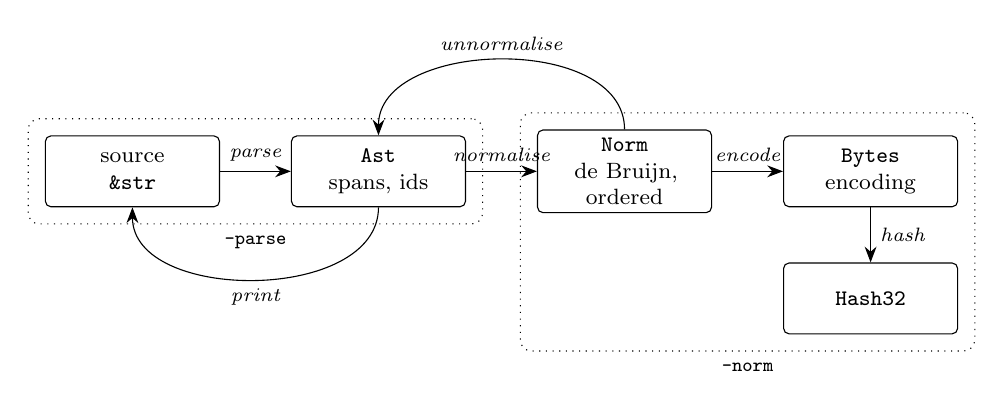
\begin{tikzpicture}[
  st/.style={draw,rounded corners=2pt,align=center,font=\footnotesize,minimum height=9mm,inner sep=3pt,text width=20mm},
  lb/.style={font=\scriptsize\itshape},
  ar/.style={-{Stealth[length=2mm]},thin}]
\node[st] (src) {source\\ \code{\&str}};
\node[st,right=9mm of src] (ast) {\code{Ast}\\ \footnotesize spans, ids};
\node[st,right=9mm of ast] (res) {\code{Norm}\\ \footnotesize de Bruijn, ordered};
\node[st,right=9mm of res] (enc) {\code{Bytes}\\ \footnotesize encoding};
\node[st,below=7mm of enc] (h) {\code{Hash32}};
\draw[ar] (src)--node[lb,above]{parse}(ast);
\draw[ar] (ast)--node[lb,above]{normalise}(res);
\draw[ar] (res)--node[lb,above]{encode}(enc);
\draw[ar] (enc)--node[lb,right]{hash}(h);
\draw[ar] (ast.south) to[out=-90,in=-90] node[lb,below]{print} (src.south);
\draw[ar] (res.north) to[out=90,in=90] node[lb,above]{unnormalise} (ast.north);
\node[draw,dotted,rounded corners,fit=(src)(ast),inner sep=6pt,label={[font=\scriptsize]below:\code{-parse}}] {};
\node[draw,dotted,rounded corners,fit=(res)(enc)(h),inner sep=6pt,label={[font=\scriptsize]below:\code{-norm}}] {};
\end{tikzpicture}
\end{center}

\code{unnormalise} takes a normal form back to a tree, with generated
identifiers in place of indices, so that a term arriving from the store or the
wire can be printed and shown. It is in \code{k1ndl1ng-norm}, since only the
normaliser knows what the indices meant.

\subsection{Composing an executive}\label{sec:executive}

An \emph{executive} is what you get when these crates are put together with a
store, a matcher and an interpreter. Nothing in this document is an executive;
this subsection exists to show that the boundaries chosen above are the ones an
executive actually wants.

\begin{center}
\begin{tabularx}{\linewidth}{@{}l>{\raggedright\arraybackslash}X@{}}
\toprule
Role & Supplied by\\
\midrule
Text to tree & \code{k1ndl1ng-parse}\\
Tree to normal form, hashes, substitution & \code{k1ndl1ng-norm}\\
Data and continuations at channels, the cut & \code{campf1r3-core}, instantiated
through \code{k1ndl1ng-campf1r3}\\
Spatial match of a pattern against a datum & the kernel matcher: a
\code{campf1r3} \code{Match} implementation over normal forms. Not specified
here; its interface is fixed by \Camp{} and its input invariants by
Section~\ref{sec:norm}\\
Choosing what runs, firing it, and the substitution that follows & the
interpreter\\
Wiring, policy, scheduling, presentation & the executive\\
\bottomrule
\end{tabularx}
\end{center}

\begin{lstlisting}
// The whole of an executive's deploy path, in outline.
let ast  = k1ndl1ng_parse::parse(src, &opts);          // or built by gesture
let term = k1ndl1ng_norm::normalise(&ast.tree, &opts)?; // de Bruijn + ordered
for p in term.top_level() {                             // rho reduces at top par
    match p.shape() {
        Shape::Send { chan, args, persistent } =>
            space.produce(chan.clone(), args.to_vec(), persistent)?,
        Shape::Receive { binds, body } =>
            space.consume(join_of(binds), pats_of(binds), cont_of(body), ...)?,
        Shape::New { .. } | Shape::Nil | Shape::Eval { .. } =>
            interpreter.handle(p)?,
    };
}
// A comm result carries a continuation and the data it matched.
// The interpreter substitutes and re-enters the loop; the store decided the race.
\end{lstlisting}

\begin{remark}[Three executives, one set of crates]
The headset executive links \code{-parse}, \code{-ast}, \code{-norm}, the
matcher, \code{campf1r3-core} and a local interpreter into one
\code{aarch64-apple-visionos} binary, with no network in the loop. The browser
demo links the same set for \code{wasm32}, replacing \Camp's \code{ExactBytes}
placeholder with real terms. The node keeps its own reducer and storage and
takes \code{k1ndl1ng-par} only, to read kernel terms into \code{Par}. The three
differ in what they wire, not in what they contain.
\end{remark}

\begin{requirement}[No executive in these crates]
No crate in this document \MUST{} contain a run loop, a scheduler, a policy for
choosing among competing communications, or a call into a store. The sketch
above is documentation, and \MAY{} ship as an example under
\code{examples/}, where it \MUST{} be feature-gated and \MUSTNOT{} be a
dependency of any library target.
\end{requirement}

%======================================================================
\section{The tree}\label{sec:ast}

\subsection{Types}

\code{k1ndl1ng-ast} defines the tree and nothing else. It is deliberately
independent of how the tree arose.

\begin{lstlisting}
pub struct Ast<'src> {
    procs:  Vec<ProcNode<'src>>,   // arena; index is ProcId
    names:  Vec<NameNode<'src>>,
    spans:  Vec<Span>,             // parallel to procs/names
    root:   ProcId,
    trivia: Vec<Trivia>,           // comments and layout, for faithful printing
}

#[derive(Clone, Copy, PartialEq, Eq)] pub struct ProcId(u32);
#[derive(Clone, Copy, PartialEq, Eq)] pub struct NameId(u32);
#[derive(Clone, Copy)] pub struct Span { pub lo: u32, pub hi: u32 }  // byte offsets

pub enum ProcNode<'src> {
    Nil,
    Par(ProcSlice),                            // flat, in source order
    Send   { chan: NameId, persistent: bool, args: ProcSlice },
    Receive{ receipt: ReceiptId, body: ProcId },
    Eval   { name: NameId },                   // *x
    New    { names: IdSlice<'src>, body: ProcId },
    Var    { id: &'src str },                  // process variable
    Wild,                                      // _
    Error  { diag: DiagId },
}

pub enum NameNode<'src> { Var { id: &'src str }, Quote(ProcId), Wild }

pub struct Receipt { pub binds: BindSlice, pub guard: Option<ProcId> }
pub struct Bind { pub kind: BindKind, pub pats: NameSlice, pub chan: NameId }
pub enum BindKind { Linear, Persistent, Peek }
\end{lstlisting}

\begin{remark}[Identifiers survive, indices do not exist yet]
\code{New} carries the declared identifiers, not a count; \code{Var} carries the
identifier text. A tree is about the program as written. Everything positional
appears one stage later, which is what lets the same tree be printed back byte
for byte.
\end{remark}

\begin{requirement}[Flat par]\label{req:flatpar}
\code{Par} \MUST{} hold a flat sequence of two or more components in source
order. The parser \MAY{} read \code{|} left-associated, but \MUSTNOT{} record a
spine of binary nodes, and \MUSTNOT{} sort. Ordering is the normaliser's
business; flatness is a property of the syntax, since $\code{|}$ is
associative and the tree shape carries no information the source had.
\end{requirement}

\begin{requirement}[Portable arithmetic]\label{req:u32}
Every index, offset, length and identifier in a public type \MUST{} be a
fixed-width type of \code{u32} or narrower, never \code{usize}, so that 32-bit
WebAssembly and 64-bit native builds agree bit for bit. A source longer than
$2^{32}-1$ bytes \MUST{} be rejected by the parser with a diagnostic.
\end{requirement}

\begin{requirement}[Arena, not pointers]
The tree \MUST{} be stored in flat vectors indexed by \code{u32}. It follows
that \code{Ast} is \code{Send}, cheap to clone in bulk, serialisable without
pointer fixups, and free of \code{Drop} recursion; the last of these is what
stops a deep term from overflowing the stack when it is released.
\end{requirement}

\begin{requirement}[No recursion anywhere]\label{req:nonrec}
Every traversal in every crate --- parsing, printing, normalisation, encoding,
substitution and \code{Drop} --- \MUST{} be iterative, driven by an explicit work
stack on the heap. No function \MUST{} recurse on term structure. The browser
main thread's stack is small, \code{stacker} is unavailable on \code{wasm32},
and a 1\,MB stack is reached by a few thousand nested quotes --- which a gesture
interface can produce by accident. A configurable \code{max\_depth} (default
$2^{16}$) \MUST{} additionally bound nesting and \MUST{} report a diagnostic
rather than abort.
\end{requirement}

\subsection{Well-formedness}

\begin{definition}[Well-formed tree]\label{def:wf}
A tree is well-formed when every \code{ProcId} and \code{NameId} is in range,
the root is reachable, every \code{Par} has at least two components, no
\code{Error} node occurs, and every \code{Span} lies within the source it was
built from, or is the null span for a constructed tree.
\end{definition}

\begin{requirement}[Well-formedness is checkable and checked]
\code{k1ndl1ng-ast} \MUST{} provide \code{Ast::check() -> Result<(), WfError>}
in $O(n)$. \code{k1ndl1ng-norm} \MUST{} either call it or document that it is
the caller's obligation, and \MUSTNOT{} have undefined behaviour on an
ill-formed tree; the worst permitted outcome is a \code{WfError}. This is the
contract that makes Requirement~\ref{req:nopar} safe for trees built by a
gesture interface rather than by the parser.
\end{requirement}

\subsection{Construction}

\begin{lstlisting}
pub struct Builder<'a> { /* arena */ }
impl<'a> Builder<'a> {
    pub fn nil(&mut self) -> ProcId;
    pub fn par(&mut self, xs: &[ProcId]) -> ProcId;
    pub fn send(&mut self, chan: NameId, persistent: bool, args: &[ProcId]) -> ProcId;
    pub fn receive(&mut self, binds: &[Bind], body: ProcId) -> ProcId;
    pub fn eval(&mut self, n: NameId) -> ProcId;
    pub fn new_names(&mut self, ids: &[&'a str], body: ProcId) -> ProcId;
    pub fn quote(&mut self, p: ProcId) -> NameId;
    pub fn name_var(&mut self, id: &'a str) -> NameId;
    pub fn finish(self, root: ProcId) -> Ast<'a>;
}
\end{lstlisting}

The builder is in \code{k1ndl1ng-ast}, not in the parser, precisely so that
\Rhobots{} can build a term from gestures and normalise it without a lexer in
the binary. A builder-produced tree \MUST{} be well-formed by construction.
%======================================================================
\section{The parser}\label{sec:parse}

\code{k1ndl1ng-parse} does one thing: text to a typed tree.

\begin{lstlisting}
pub struct Options { pub level: Level, pub max_depth: u32, pub desugar_seq: bool }
pub enum Level { K0, K1, K2 }

pub fn parse<'src>(src: &'src str, opts: &Options) -> Parsed<'src>;
pub struct Parsed<'src> { pub tree: Ast<'src>, pub diags: Vec<Diag> }

/// Parse one process, for splicing into an existing tree.
pub fn parse_fragment<'src>(src: &'src str, opts: &Options) -> Parsed<'src>;
\end{lstlisting}

\begin{center}
\begin{tabularx}{\linewidth}{@{}l>{\raggedright\arraybackslash}X@{}}
\toprule
Stage & What it does and does not do\\
\midrule
Lexer & One left-to-right pass, no backtracking, no regular expressions. Tokens
carry a kind and a byte range and nothing else; text is recovered by slicing the
source. Trivia is recorded in a side table, not in the token stream.\\
Parser & Explicit-stack descent (Requirement~\ref{req:nonrec}) producing
\code{Ast}: arena nodes, \code{u32} indices, spans, node identifiers.
Identifiers are \code{\&str} borrowed from the source. No binder analysis, no
ordering, no equality, no desugaring beyond sequential receipts.\\
\bottomrule
\end{tabularx}
\end{center}

\begin{requirement}[The parser has no opinion about binding]\label{req:noopinion}
The parser \MUST{} accept a syntactically valid term whose variables are
unbound, duplicated in a pattern, or shadowed. Those are diagnostics of
Section~\ref{sec:binders}, produced by the normaliser. An editor showing a
half-written term needs a tree for it; refusing to build one is the behaviour
that makes structure editing impossible.
\end{requirement}

\begin{decision}[Sequential receipts are the one desugaring]
\code{for(a <- x; b <- y)\{P\}} is parsed as nested receives when
\code{desugar\_seq} is set, and as a single receive node with two receipts when
it is not. Default is set. This is the only sugar in the kernel, and the flag
exists so that a formatter can round-trip the source form while an executive
sees only the nested form. If the flag proves a nuisance, the honest
alternative is to drop \code{;} from the kernel entirely.
\end{decision}

\begin{requirement}[Level is a parser parameter]\label{req:level2}
The parser \MUST{} take the accepted level (Section~\ref{sec:lang}) as an
explicit parameter, \MUST{} reject forms above that level with a diagnostic
naming the level that would accept them, and \MUSTNOT{} silently accept them.
K0 and K1 \MUST{} be implemented in v1; K2 \MUST{} be behind the \code{guards}
cargo feature, off by default.
\end{requirement}

%======================================================================
\section{The normaliser}\label{sec:norm}

\code{k1ndl1ng-norm} takes a well-formed tree to a normal form: de Bruijn
indices for bound occurrences, de Bruijn levels for free ones, ordered parallel
components, and the encoding and content hash that follow. Name equality then
costs a 32-byte comparison, which is the point of the exercise.

\begin{lstlisting}
pub fn normalise(tree: &Ast<'_>, opts: &Options) -> Result<Norm, Vec<Diag>>;
pub fn unnormalise(t: &Norm) -> Ast<'static>;          // for printing and display

impl Norm {
    pub fn encode(&self) -> &[u8];                     // memoised
    pub fn hash<D: Digest32>(&self) -> Hash32;         // memoised
    pub fn decode(bytes: &[u8]) -> Result<Norm, DecodeError>;
    pub fn substitute(&self, env: &Subst) -> Norm;     // Decision 1.7
    pub fn shift(&self, by: i32, cutoff: u32) -> Norm;
    pub fn top_level(&self) -> &[Norm];                // the par components
    pub fn free_names(&self) -> &[FreeName];
    pub fn size(&self) -> u32;
    pub fn depth(&self) -> u32;
}
\end{lstlisting}

\subsection{Binders}\label{sec:binders}

Rho has two binding forms and one derived one. \code{for} binds names in its
patterns; \code{new} binds names in its body; a quoted pattern
\code{@\{\ldots x \ldots\}} binds the process variable $x$ at the position of the
enclosing name pattern.

\begin{definition}[Sorts]
An identifier occurrence resolves to exactly one of: \code{NameBound(i)} --- a
bound name, de Bruijn index $i$; \code{ProcBound(i)} --- a process variable
bound by a quoted pattern; \code{FreeName(l)} / \code{FreeProc(l)} --- free,
carrying the de Bruijn level of its first occurrence.
\end{definition}

\begin{requirement}[Static checks belong here]\label{req:static}
The normaliser \MUST{} reject, with a diagnostic and the span carried by the
tree: (i) a free variable occurring twice in one pattern; (ii) a wildcard where
a bound occurrence is required (\code{*\_}); (iii) a \code{new}-bound name used
as a pattern variable; (iv) a term with free names, when the caller asked for a
closed term. It \MUSTNOT{} reject free names otherwise.
\end{requirement}

\begin{decision}[Free names are reported, not an error]\label{dec:free}
\code{Norm} carries \code{free\_names} in first-occurrence order, with the
identifier and span from the tree. \Rhobots{} synthesises its canonical outer
comprehension on \code{stdin} from exactly this list; the node adapter uses it to
decide whether a term is deployable. The normaliser takes no view. This differs
deliberately from \code{f1r3node}'s \code{source\_to\_adt}, which errors when
\code{free\_map.count() > 0}, and the difference \MUST{} be documented where the
two meet.
\end{decision}

\subsection{Unforgeable names}

\code{new} introduces names that quote nothing. \code{Norm} represents them as
\code{Name::Unforgeable}, carrying 32 bytes minted through a trait rather
than by a fixed scheme:

\begin{lstlisting}
pub trait NameMinter { fn mint(&mut self, path: &BinderPath) -> [u8; 32]; }
pub struct Sequential;     // pure function of binder position; the default
\end{lstlisting}

\begin{decision}[Minting is the caller's policy]
\code{Sequential} is a pure function of the binder's position in the normal
form, so a \Kind-only pipeline is deterministic and reproducible. It is
\emph{not} compatible with \code{f1r3node}'s deploy-seeded derivation and
\MUSTNOT{} be presented as such; \code{k1ndl1ng-par} supplies a minter that
reproduces the node's scheme, so compatibility is a property of the adapter,
tested differentially, and not a constraint on the core.
\end{decision}

\subsection{The normal form and its encoding}

\begin{definition}[Encoding]\label{def:enc}
$\enc{-}$ maps a normal form to a byte string. Each constructor is a tag byte
followed by its fields; lengths are LEB128-encoded \code{u32}; identifiers never
appear, only de Bruijn indices and levels.
\end{definition}

\begin{center}
\begin{tabular}{@{}llll@{}}
\toprule
Tag & Constructor & Payload & Ordered\\
\midrule
\code{0x00} & \code{Nil} & --- & ---\\
\code{0x01} & \code{Par} & $n$, then $\enc{P_1}\cdots\enc{P_n}$ & yes, by $\enc{P_i}$\\
\code{0x02} & \code{Send} & $\enc{x}$, persistence bit, $n$, $\enc{Q_1}\cdots\enc{Q_n}$ & no (arity is ordered)\\
\code{0x03} & \code{Receive} & $m$, $\enc{b_1}\cdots\enc{b_m}$, $\enc{P}$ & yes, by $\enc{b_j}$\\
\code{0x04} & \code{New} & $k$, $\enc{P}$ & ---\\
\code{0x05} & \code{Eval} & $\enc{x}$ where $x$ is a variable & ---\\
\code{0x06} & \code{BoundVar} & index & ---\\
\code{0x07} & \code{FreeVar} & level & ---\\
\code{0x08} & \code{Wild} & --- & ---\\
\code{0x10} & \code{Quote} & $\enc{P}$ & ---\\
\code{0x11} & \code{BoundName} & index & ---\\
\code{0x12} & \code{FreeName} & level & ---\\
\code{0x13} & \code{Unforgeable} & 32 bytes & ---\\
\code{0x20} & \code{Bind} & kind byte, $\enc{\text{chan}}$, $n$, patterns & no\\
\bottomrule
\end{tabular}
\end{center}

\begin{requirement}[The order key is the encoding itself]\label{req:sortkey}
Parallel components and the binds of one receipt \MUST{} be ordered by bytewise
lexicographic comparison of their own encodings, ascending. No separate score
tree is computed, and no ordering \MUST{} depend on source order, hash values,
pointer values or iteration order of a hash container.
\end{requirement}

\begin{remark}[Why not the node's score tree]
\code{models}'s sorter builds a score tree per term, sorts by it, and serialises
separately, and in \code{f1r3node} the sort is a pass distinct from
normalisation, invoked at substitution and storage time. For the kernel the
encoding \emph{is} a score tree, flattened: tags are assigned in the order the
sorter's \code{Score} constants assign them, so bytewise comparison agrees with
score comparison on this fragment, and one pass does the work of two. Agreement
with \code{models} is an obligation, not an assumption
(Obligation~\ref{obl:sortagree}).
\end{remark}

\begin{requirement}[Bottom-up, memoised]
Normalisation \MUST{} compute each subterm's encoding once, bottom-up, and
\MUST{} reuse it as the order key of the parent, so that ordering a par of $n$
components of size $s$ costs $O(n\log n\cdot s)$ comparisons of already-built
byte strings and not $O(n\log n)$ re-encodings.
\end{requirement}

\subsection{Correctness}

\begin{proposition}[Normal form decides congruence]\label{prop:decides}
For kernel terms $P,Q$ with the same free-name environment,
$\enc{P}=\enc{Q}$ iff $P\equiv Q$, with $\equiv$ as in
Definition~\ref{def:cong}.
\end{proposition}
\begin{proof}[Proof sketch]
($\Leftarrow$) By induction on the derivation of $\equiv$. Commutativity and
associativity of \code{|} are absorbed by flatness
(Requirement~\ref{req:flatpar}) and by Requirement~\ref{req:sortkey}, since a
total order on encodings gives one representative per multiset. \code{Nil} as
unit is absorbed by dropping \code{Nil} components during normalisation, except
for the empty par, which encodes as \code{0x00}. $\alpha$-equivalence is
absorbed by de Bruijn indices, assigned by position and not by name.
$*@P \equiv P$ and $@{*x} \equiv_N x$ are absorbed by two rewrites applied during
normalisation, confluent and terminating since each strictly decreases the count
of $*@$ and $@*$ pairs. ($\Rightarrow$) By induction on the length of the
encoding: the tag determines the constructor and LEB128 lengths determine field
boundaries, so decoding is a function; the decoded term is congruent to any term
with that encoding by the first direction applied to the representative.
\end{proof}

\begin{requirement}[Idempotence and stability]
\code{normalise} \MUST{} be idempotent through \code{unnormalise}, and \MUST{}
be invariant under permutation of the components of a par in the tree. Both
\MUST{} be property tested (Section~\ref{sec:testing}).
\end{requirement}

\begin{obligation}[Free levels and ordering interact]\label{obl:levels}
Levels are assigned by first occurrence in a left-to-right traversal, and
ordering reorders the traversal. The implementation \MUST{} therefore assign
levels \emph{after} ordering, in a traversal of the ordered term, and \MUST{}
reach a fixed point: order with the previous round's levels, reassign, repeat.
Two rounds suffice for the kernel; that claim is recorded here as an obligation
to be proved or replaced by a loop with a proved bound. The same subtlety exists
in \code{models} and is worth checking there.
\end{obligation}

\begin{obligation}[Agreement with the node's normaliser and sorter]\label{obl:sortagree}
For every kernel term, the \code{Norm} produced here and the \code{Par} produced
by \code{Compiler::source\_to\_adt} followed by \code{ParSortMatcher} \MUST{}
induce the same channel identity: equal terms give equal \code{Blake2b-256}
hashes under the node's serialisation. Established by differential test over the
corpus, not by construction, because the two encodings differ.
\end{obligation}

\subsection{Hashing}

\begin{lstlisting}
pub struct Hash32(pub [u8; 32]);
pub trait Digest32 { fn digest(bytes: &[u8]) -> Hash32; }
pub struct Blake2b256;              // default, in-crate, ~200 lines, no C
\end{lstlisting}

\begin{requirement}[Hash discipline, caller side]
\code{k1ndl1ng-norm} \MUST{} compute the content hash of a term exactly once,
from $\enc{-}$, and \MUST{} expose it so that a \Camp{} caller satisfies that
store's \code{Keyed} contract without re-serialising. The digest \MUST{} be a
type parameter with \code{Blake2b256} as default. The implementation \MUSTNOT{}
use a C library or a crate outside the allowlist of Section~\ref{sec:wasm}.
\end{requirement}

%======================================================================
\section{Instantiating \Camp}\label{sec:glue}

\code{k1ndl1ng-campf1r3} is the only crate that names both projects. It contains
type definitions and trait implementations, and \SHOULD{} contain no algorithm.

\begin{center}
\begin{tabularx}{\linewidth}{@{}l>{\raggedright\arraybackslash}X@{}}
\toprule
\Camp{} parameter & Instantiated at\\
\midrule
\code{C} (channel) & \code{Name} in normal form: a quoted \code{Norm}, a free
name level, or an unforgeable identifier. \code{content\_hash} is the memoised
hash of its encoding.\\
\code{A} (datum) & \code{Norm}. The send's argument list becomes the datum
sequence, so \Camp's arity check is the send's arity.\\
\code{P} (pattern) & \code{Pattern}: a \code{Norm} whose free variables and
wildcards are the binding sites, with the binder count precomputed.\\
\code{K} (continuation) & \code{Cont \{ body: Norm, binders: u16 \}}, hashed over
the body encoding together with the binder count.\\
Matcher & \emph{not supplied here.} The kernel matcher is a separate
deliverable; this specification guarantees only that patterns and data are in
normal form when it is called, which is what makes a linear-time structural
match possible.\\
\bottomrule
\end{tabularx}
\end{center}

\begin{remark}[What this buys the store]
\Camp{} forbids itself from hashing payloads, and notes that \code{rspace++}
today serialises and hashes every candidate on every produce and consume. With
the normaliser, the hash is computed once when the term is built and carried
with it, so the matching loop compares 32 bytes to reject and calls the matcher
only on survivors.
\end{remark}

\subsection{The WebAssembly interface}

\code{k1ndl1ng-wasm} exposes each crate behind a cargo feature, at the byte
level, so that neither the JS nor the Swift side owns a Rust object graph, and a
module that only parses does not carry a normaliser.

\begin{lstlisting}
// feature = "parse"
#[wasm_bindgen] pub fn parse_to_tree(src: &str, level: u8) -> Box<[u8]>;   // tree wire form
#[wasm_bindgen] pub fn diagnostics(src: &str, level: u8) -> String;        // JSON
#[wasm_bindgen] pub fn print_tree(tree: &[u8], style: u8) -> String;
// feature = "norm"
#[wasm_bindgen] pub fn normalise(tree: &[u8]) -> Box<[u8]>;                // normal form
#[wasm_bindgen] pub fn hash_of(norm: &[u8]) -> Box<[u8]>;                  // 32 bytes
#[wasm_bindgen] pub fn scene(norm: &[u8]) -> Box<[u8]>;                    // Section 10.4
\end{lstlisting}

\begin{requirement}[No stub builds]\label{req:nostub}
A \code{wasm32} build \MUSTNOT{} substitute a reduced or empty implementation of
any function in this specification. If a target cannot support a feature, the
build \MUST{} fail at compile time. The precedent to avoid is explicit:
\code{rholang-parser}'s \code{wasm32} stub returns a successful parse of the
empty process for every input.
\end{requirement}

\begin{requirement}[Total functions]\label{req:total}
No public function in any crate \MUST{} panic, abort, or call \code{unwrap} on
input-derived data, for any input byte string, including invalid UTF-8
boundaries, unbalanced delimiters, 4\,GB of open parentheses, an ill-formed
tree, a truncated encoding, and adversarially deep nesting. This \MUST{} be
established by fuzzing (Section~\ref{sec:testing}) and \MUST{} be a release
gate. \code{unsafe} \MUSTNOT{} appear in any crate.
\end{requirement}
%======================================================================
\section{Errors and recovery}\label{sec:errors}

\begin{requirement}[Diagnostics, not exceptions]
Every failure \MUST{} be a \code{Diag} in a list, with a \code{Span}, a stable
\code{code}, a severity, and an optional primary suggestion. Parsing \MUST{}
continue after a syntax error and \MUST{} report every independent error in one
pass, because an editor that shows one error at a time teaches the programmer to
compile repeatedly. Normalisation \MUST{} likewise accumulate binding errors
rather than stopping at the first.
\end{requirement}

\begin{lstlisting}
pub struct Diag { pub code: Code, pub span: Span, pub sev: Sev, pub note: Option<Note> }
pub enum Sev { Error, Warning }
\end{lstlisting}

\code{Diag}, \code{Code} and \code{Span} live in \code{k1ndl1ng-ast}, so that a
consumer can handle diagnostics from both crates uniformly. The code set is
closed, and each group belongs to exactly one crate:

\begin{center}
\begin{tabularx}{\linewidth}{@{}ll>{\raggedright\arraybackslash}X@{}}
\toprule
Group & Raised by & Codes\\
\midrule
Lexical & \code{-parse} & \code{UnknownByte}, \code{UnterminatedComment},
\code{NonAsciiIdent}, \code{SourceTooLarge}\\
Syntax & \code{-parse} & \code{Expected}, \code{Unbalanced},
\code{EmptySend}, \code{MissingBody}, \code{TooDeep}\\
Level & \code{-parse} & \code{NotInKernel}, \code{NeedsK1}, \code{NeedsK2},
\code{ArityAtK0}\\
Well-formedness & \code{-ast} & \code{BadId}, \code{Unreachable},
\code{DegeneratePar}, \code{SpanOutOfRange}\\
Binding & \code{-norm} & \code{DuplicatePatternVar},
\code{WildcardNotBindable}, \code{UnboundRequired}, \code{NewNameInPattern}\\
Encoding & \code{-norm} & \code{DecodeTruncated}, \code{DecodeBadTag},
\code{DecodeBadIndex}\\
\bottomrule
\end{tabularx}
\end{center}

\begin{requirement}[Recovery is structural]
Recovery \MUST{} be by synchronisation on the kernel's delimiters ---
\code{\}}, \code{)}, \code{|} at the current nesting depth --- and the damaged
region \MUST{} be recorded as a \code{ProcNode::Error} covering its span, so the
tree remains a tree over the whole source. A tree containing \code{Error} nodes
\MUST{} still print and \MUST{} still support editor queries; it is not
well-formed (Definition~\ref{def:wf}), so \code{normalise} \MUST{} refuse it and
return the diagnostics that produced it.
\end{requirement}

\begin{requirement}[Level diagnostics name the level]
A construct rejected only because of the accepted level \MUST{} report
\code{NeedsK1} or \code{NeedsK2} and \MUSTNOT{} report a syntax error. The
editor uses this to offer ``this term needs the store kernel'' rather than
``unexpected token''.
\end{requirement}

%======================================================================
\section{Editor services}\label{sec:editor}

These exist because \Rhobots{} needs them, and are specified here rather than in
the visionOS client so that a text editor, an LSP server and the headset share
one implementation. They are split by crate on the same principle as everything
else: anything about the source is in \code{-parse}, anything about the tree is
in \code{-ast}, anything that needs identity is in \code{-norm}.

\subsection{Stable identity}

\begin{requirement}[Node identity survives edits]\label{req:ids}
\code{k1ndl1ng-ast} \MUST{} expose \code{NodeId}s stable across a reparse of an
unchanged subtree, so that a robot in the scene keeps its position, animation
state and physical continuity when the programmer edits a sibling. Identity
\MUST{} be computed as a function of the path from the root together with the
hash of the subtree's normal form, and \MUSTNOT{} be a counter over allocation
order.
\end{requirement}

\begin{remark}[The one place the split costs something]
That definition needs the normaliser, which \code{-ast} may not depend on
(Requirement~\ref{req:acyclic}). The resolution: \code{-ast} defines
\code{NodeId} and an \code{Identify} trait with a path-only default;
\code{-norm} provides the hash-backed implementation. An editor that links only
the parser gets identity stable under sibling edits but not under a renaming;
one that links both gets the full guarantee. \Rhobots{} links both.
\end{remark}

\subsection{Subterm reparse and splice}

\begin{lstlisting}
// k1ndl1ng-parse
pub fn parse_fragment<'s>(src: &'s str, opts: &Options) -> Parsed<'s>;
// k1ndl1ng-ast
pub fn splice(tree: &Ast<'_>, at: ProcId, frag: &Ast<'_>) -> Ast<'static>;
pub fn subtree_source<'s>(tree: &Ast<'s>, at: ProcId) -> &'s str;   // by span
\end{lstlisting}

\begin{decision}[No incremental parsing in v1]
Incremental reparse is the tree-sitter feature most obviously lost, and it is
not missed. \Rhobots{} edits structure, not text: a gesture builds a node, and
\code{Builder} serves that directly. Where text is typed, it is typed into one
subterm, and \code{parse\_fragment} plus \code{splice} reparses that subterm
only. Whole-file incremental parsing is reconsidered if the LSP server, not the
headset, asks for it.
\end{decision}

\subsection{Printing}

\begin{lstlisting}
// k1ndl1ng-ast
pub fn print(tree: &Ast<'_>, style: &PrintStyle) -> String;   // Faithful | Plain
// k1ndl1ng-norm
pub fn print_norm(t: &Norm, style: &PrintStyle) -> String;    // via unnormalise
\end{lstlisting}

\begin{requirement}[Round trip]\label{req:roundtrip}
For every well-formed tree $a$, \code{parse(print(a, Plain))} \MUST{} yield a
tree with the same normal form. For every source $s$ that parses cleanly,
\code{print(parse(s).tree, Faithful)} \MUST{} reproduce $s$ byte for byte,
including comments and layout. For every normal form $t$,
\code{normalise(unnormalise(t))} \MUST{} equal $t$. All three \MUST{} be
property tested.
\end{requirement}

\begin{remark}[Why two printing styles and not three]
\code{Faithful} prints from the tree with its trivia table, and is what an
editor writes back to a file when only part of the term was touched.
\code{Plain} prints the tree in the crate's own layout, discarding trivia, and
is what the headset exports. A printed \emph{normal form} is just
\code{Plain} applied to \code{unnormalise}, so there is no third style: the
stability that used to be called ``canonical printing'' is a property of the
normal form, not of the printer.
\end{remark}

\subsection{Scene queries}

\begin{lstlisting}
// k1ndl1ng-norm
pub fn top_level(t: &Norm) -> &[Norm];        // what can act now: the z=0 plane
pub fn continuation_of(t: &Norm) -> Option<&Norm>;  // what sits behind a receive
pub fn free_names(t: &Norm) -> &[FreeName];
pub fn metrics(t: &Norm) -> Metrics;          // size, depth, width per node
pub fn redex_candidates(t: &Norm) -> Vec<(u32, u32)>;
\end{lstlisting}

\begin{requirement}[Candidates are syntactic]
\code{redex\_candidates} \MUST{} report pairs of a top-level send and a
top-level receive whose channels are equal as normal-form names --- a hash
comparison. It \MUSTNOT{} perform pattern matching, decide a race, or reduce.
\Rhobots{} uses it to decide which robots walk toward each other; the store
decides what actually fires.
\end{requirement}

\begin{remark}[Level of detail]
\code{metrics} exists so the renderer can decide when a shrunken robot falls
below legibility and is replaced by the elision glyph the \Rhobots{} spec calls
for. Size and depth are computed during normalisation at no extra traversal.
\end{remark}

%======================================================================
\section{Performance}\label{sec:perf}

\subsection{Complexity}

Let $n$ be source bytes, $m$ the node count, $w$ the width of the widest par,
$d$ the depth, $s$ the mean encoded subterm size.

\begin{center}
\begin{tabular}{@{}llll@{}}
\toprule
Crate & Stage & Time & Space\\
\midrule
\code{-parse} & lex & $O(n)$, one pass & reused token buffer\\
\code{-parse} & parse & $O(n)$ & $O(m)$ arena $+$ $O(d)$ work stack\\
\code{-norm} & resolve & $O(m)$ & $O(d)$ scope stack\\
\code{-norm} & order $+$ encode & $O(m + \sum w\log w\cdot s)$ & $O(m)$ shared encodings\\
\code{-norm} & hash & $O(|\enc{-}|)$ & $O(1)$\\
\code{-norm} & substitute & $O(m)$ & $O(m)$\\
\code{-ast} & print & $O(m + \text{output})$ & $O(d)$\\
\bottomrule
\end{tabular}
\end{center}

\subsection{Targets}

Measured on the reference platform (\code{aarch64} macOS, one thread) over a
corpus of kernel terms derived from \code{rholang-parser/tests/corpus} plus
generated terms.

\begin{center}
\begin{tabularx}{\linewidth}{@{}l>{\raggedright\arraybackslash}X@{}}
\toprule
Quantity & Target\\
\midrule
Parse throughput & $\ge 40$\,MiB/s native; $\ge 15$\,MiB/s under \code{wasm32}\\
Normalise $+$ hash & $\ge 100$\,MiB/s of encoding\\
Small term latency & $\le 2\,\mu$s from text to hashed normal form for a term
under 200 bytes; this is the \Rhobots{} keystroke budget and the \Camp{} deploy
budget\\
Allocation & $O(1)$ arena growth events per parse; zero allocation per token;
peak heap $\le 8n$\\
Code size, \code{-parse} $+$ \code{-ast} & $\le 80$\,KiB uncompressed in a
\code{wasm32} module, against 2.75\,MB of generated C in the component it
replaces\\
Code size, \code{-norm} & $\le 60$\,KiB uncompressed, so that a parse-only
module is genuinely smaller than a full one and the split earns its keep\\
Cold start & $\le 1$\,ms to first parse in a fresh WebAssembly instance; no lazy
table construction, no global initialisation\\
\bottomrule
\end{tabularx}
\end{center}

\begin{requirement}[Benchmarks are a gate]
A benchmark suite \MUST{} run in CI on the reference platform, per crate, and
\MUST{} fail the build on a regression of more than 10\% against the recorded
baseline. Code size \MUST{} be measured the same way, for each of the two
WebAssembly feature sets separately. Targets above are stated relative to
measurements, and the first task of phase~1 is to record the baseline, including
the current tree-sitter parser's throughput on the same corpus.
\end{requirement}
%======================================================================
\section{Portability, determinism and dependencies}\label{sec:wasm}

\begin{center}
\begin{tabularx}{\linewidth}{@{}lc>{\raggedright\arraybackslash}X@{}}
\toprule
Target & Level & Notes\\
\midrule
\code{x86\_64}/\code{aarch64} Linux, macOS & \MUST & Reference platforms.\\
\code{wasm32-unknown-unknown} & \MUST & Browser and \Camp{} demo; no stubs
(Requirement~\ref{req:nostub}).\\
\code{aarch64-apple-visionos} (and simulator) & \MUST & \Rhobots, through a C
ABI or a Swift package wrapping the static library.\\
\code{wasm32-wasip1} & \SHOULD & Non-browser hosts.\\
\code{no\_std} $+$ \code{alloc} & \SHOULD & Achievable for all three core
crates; the only \code{std} uses are \code{String} in printing and \code{Vec}.\\
\bottomrule
\end{tabularx}
\end{center}

\begin{requirement}[Dependency allowlist]\label{req:deps}
\code{k1ndl1ng-ast}, \code{k1ndl1ng-parse} and \code{k1ndl1ng-norm} \MUST{}
build with \code{core} and \code{alloc} and, at most, \code{smallvec}, plus the
one intra-family dependency each is permitted in Section~\ref{sec:arch}. They
\MUSTNOT{} depend, directly or transitively, on \code{tree-sitter} or any C
library, \code{serde}, \code{bincode}, \code{prost}, \code{regex},
\code{getrandom}, \code{tokio}, \code{rayon}, \code{lazy\_static}, or any crate
of the \code{f1r3node-rust} or \code{rholang-rs} workspaces.
\code{k1ndl1ng-wasm} \MAY{} add \code{wasm-bindgen}. An optional \code{serde}
feature \MAY{} derive encodings for \code{Diag} and \code{Metrics} only, never
for \code{Norm}, whose encoding is normative.
\end{requirement}

\begin{requirement}[Determinism]\label{req:det}
For one input and one \code{Options}, the tree, the normal form, its encoding,
the content hash, the diagnostic list in order, and both printings \MUST{} be
identical bit for bit across targets, pointer widths, optimisation levels and
toolchain versions within the supported MSRV range. No output \MUST{} depend on
hash-map iteration order, address values, floating point, locale, or time. Hash
containers \MUSTNOT{} appear on any path affecting output order; where a map is
needed it \MUST{} be a sorted structure or keyed by a deterministic index.
\end{requirement}

\begin{remark}
Requirement~\ref{req:det} is the normaliser's half of \Camp's determinism
profiles. A \code{Deterministic} store fed by a non-deterministic front end is
not deterministic, and replay would diverge at the first term whose components
were ordered differently on two machines.
\end{remark}

\begin{requirement}[MSRV, versioning and the wire forms]
Each crate \MUST{} declare an MSRV and hold it for the life of a minor version;
\MUST{} be \code{\#![forbid(unsafe\_code)]}; and \MUST{} version independently.
Two byte formats are part of the public interface and \MUST{} each carry a
one-byte format tag, changed only on a major version: the normal-form encoding
of Section~\ref{sec:norm}, and the tree wire form used by
\code{k1ndl1ng-wasm}. A change to the encoding changes every content hash, and
therefore every channel identity in every store built with it; it is the most
expensive change this family can make.
\end{requirement}

%======================================================================
\section{Validation}\label{sec:testing}

\begin{center}
\begin{tabularx}{\linewidth}{@{}ll>{\raggedright\arraybackslash}X@{}}
\toprule
Kind & Crate & Content\\
\midrule
Golden corpus & all & Every kernel term in \code{rholang-parser/tests/corpus}
plus a kernel-specific corpus; snapshots of tree, normal form, encoding, hash
and both printings.\\
Round trip & \code{-ast}, \code{-parse}, \code{-norm} & The three properties of
Requirement~\ref{req:roundtrip}, over generated terms and over the corpus.\\
Congruence & \code{-norm} & Generate $P$, apply random congruence-preserving
rewrites (commute a par, $\alpha$-rename, insert and remove \code{Nil}, wrap and
unwrap $*@$), assert equal encodings; generate distinct terms, assert distinct
encodings. This tests Proposition~\ref{prop:decides} in both directions.\\
Builder parity & \code{-ast} & A tree built through \code{Builder} and the same
tree parsed from its own \code{Plain} printing \MUST{} normalise identically.
This is the gate on Requirement~\ref{req:nopar}, and the gate on \Rhobots{}
gesture editing.\\
Independence & all & A build of \code{-parse} with \code{-norm} absent, and of
\code{-norm} with \code{-parse} absent, \MUST{} both succeed and pass their own
suites. Checked in CI, because a dependency creeps in by accident, never on
purpose.\\
Differential, syntax & \code{-parse} & Parse the corpus with
\code{rholang-parser} and with \Kind; assert the trees agree on the kernel
fragment and that every form \Kind{} rejects is either outside the kernel or
rejected by both.\\
Differential, identity & \code{-par} & For each corpus term, compare the
normaliser's hash with the \code{Blake2b-256} of the node's sorted \code{Par};
this discharges Obligation~\ref{obl:sortagree}.\\
Differential, store & \code{-campf1r3} & Drive \Camp{} with normal-form terms
and with the \code{ExactBytes} reference instantiation over the same scripted
operation sequence; assert identical event logs.\\
Fuzzing & \code{-parse}, \code{-norm} & \code{cargo-fuzz} targets for
\code{parse}, \code{normalise} on an arbitrary tree, \code{Norm::decode} and
\code{splice}; the gate for Requirement~\ref{req:total} is 24 hours clean per
release.\\
Cross-target & all & Run the golden corpus under \code{wasm32} in a host and
compare byte for byte with native output; the gate for
Requirement~\ref{req:det}.\\
\bottomrule
\end{tabularx}
\end{center}

%======================================================================
\section{Open decisions}\label{sec:open}

\begin{enumerate}[leftmargin=1.8em,nosep]
\item \textbf{Name.} \Kind{} is the working name for the family: kindling is
what you feed a campfire. Crate names \code{k1ndl1ng-ast},
\code{k1ndl1ng-parse}, \code{k1ndl1ng-norm} follow from it. Decide before the
repository is created.
\item \textbf{One repository or three.} The three core crates can share a cargo
workspace and a version cadence, or live separately. A workspace is recommended:
it makes the independence test of Section~\ref{sec:testing} a CI job rather than
an act of faith, while the crates still publish and version separately.
\item \textbf{Whether \code{-ast} is its own crate.} Folding it into
\code{-parse} would leave two crates rather than three, at the cost of making a
gesture-built tree depend on a lexer --- which is exactly the dependency
Requirement~\ref{req:nopar} exists to prevent. Keeping it separate is
recommended, and is cheap: it has no dependencies and almost no logic.
\item \textbf{Guards at K2.} Whether \code{where} clauses are in v1 at all.
Recommended: parse them behind a feature, carry the guard as an unevaluated
subterm through normalisation, and let the executive hand it to
\code{rho-pure-eval}. No crate here evaluates anything.
\item \textbf{\code{new} at K1.} Pure rho does not need it and \Rhobots{}
excludes it; it is included because a store kernel without unforgeable names
cannot express a private channel. If kernel terms are never deployed directly,
\code{new} moves to K2 and the normaliser shrinks.
\item \textbf{Polyadic at K0.} K0 is monadic here, following \emph{Rhobots in
Space}. If the renderer would rather draw a robot with $n$ hands from the start,
K0 becomes polyadic and one level's worth of checking disappears.
\item \textbf{The kernel matcher.} A spatial matcher over normal-form patterns
is the remaining piece between this family and \Camp, and the piece that makes a
headset-local executive possible. It is out of scope here. Whether it is
\code{k1ndl1ng-match} or a \Camp{} companion is a question about which
repository owns pattern semantics; its input invariants are already fixed by
Section~\ref{sec:norm}.
\item \textbf{The interpreter.} Likewise unspecified, and likewise the executive
cannot be built without it. It needs only \code{-norm} and a store, and
Decision~\ref{dec:subst} is what keeps it from reimplementing de Bruijn
arithmetic.
\end{enumerate}

%======================================================================
\section{Delivery}\label{sec:delivery}

Six phases, each ending in something runnable.

\begin{enumerate}[leftmargin=1.8em,nosep]
\item \textbf{Baseline and tree.} Workspace, CI, benchmark harness, recorded
baseline measurements of \code{rholang-parser} on the shared corpus.
\code{k1ndl1ng-ast} complete: types, arena, builder, well-formedness check,
both printings.
\item \textbf{K0 parser.} \code{k1ndl1ng-parse} at K0: lexer, parser,
diagnostics, recovery, fragment and splice; faithful round trip. At the end of
this phase an editor can load, show and write pure rho.
\item \textbf{K0 normaliser.} \code{k1ndl1ng-norm} at K0: binders, ordering,
encoding, \code{Blake2b256}, \code{unnormalise}, substitution; congruence and
builder-parity property tests. At the end of this phase name equality is a hash
comparison and \Rhobots{} has everything it needs from this family.
\item \textbf{WebAssembly.} \code{k1ndl1ng-wasm} with the two feature sets,
cross-target determinism tests, per-feature code-size gates.
\item \textbf{K1 and the store.} Joins, persistence, peek, polyadic, patterns,
\code{new}, sequential-receipt sugar, in both crates; then
\code{k1ndl1ng-campf1r3} and the store differential test. At the end of this
phase \Camp{} in a browser runs on real terms instead of \code{ExactBytes}.
\item \textbf{Node adapter and K2.} \code{k1ndl1ng-par} in the
\code{f1r3node-rust} workspace, the identity differential test
(Obligation~\ref{obl:sortagree}), the node-compatible minter; then \code{where}
guards behind the feature, if Section~\ref{sec:open}(4) says so.
\end{enumerate}

\vfill
\noindent\rule{\linewidth}{0.4pt}\\[2pt]
\footnotesize
Facts about existing code in this document were read from
\code{F1R3FLY-io/f1r3node-rust} at branch \code{feature/cost-accounted-rho} and
\code{F1R3FLY-io/rholang-rs} at \code{master}, on 17 September 2026.

\end{document}
